\chapter{Examples} \label{chap:examples}
results text...

\section{2D-problem A: XOR function} \label{sec:dataset_xor}
The standard Exclusive OR (XOR) function is defined by truth \cref{tab:examples:xor_function}. Based on this function one can set a classification problem with two features and two classes.

\begin{table}[H]
\centering
\begin{tabular}{|c|c||c|}
\hline
\textit{$ x_1 $} & \textit{$ x_2 $} & \textit{y} \\ \hline \hline
0                & 0                & 0          \\ \hline
0                & 1                & 1          \\ \hline
1                & 0                & 1          \\ \hline
1                & 1                & 0          \\ \hline
\end{tabular}
\caption{Standard XOR function.}
\label{tab:examples:xor_function}
\end{table}

This problem serves perfectly for demonstration of network optimization methods, as two optimal architectural solutions producing the XOR function are known (\cref{fig:examples:xor_solutions}). 

\begin{figure}[H]
\centering
\begin{subfigure}{.4\textwidth}
  \centering
  \includegraphics[height=2cm]{xor_min1}
  \caption{Solution in 2D.}
  \label{fig:examples:xor_min1}
\end{subfigure}
\begin{subfigure}{.4\textwidth}
  \centering
  \includegraphics[height=2cm]{xor_min2}
  \caption{Solution in 3D.}
  \label{fig:examples:xor_min2}
\end{subfigure}
\caption{Optimal network architectures producing the XOR function.}
\label{fig:examples:xor_solutions}
\end{figure}

With this knowledge we can proove that the pruning algorithm is (or is not) able to find the optimal solution. If the method is correct, it should end up with one of the shown architectures (\cref{fig:examples:xor_min1} or \cref{fig:examples:xor_min2}).

The truth \cref{tab:examples:xor_function} ruled the generation of a 2D dataset illustrated in \cref{fig:examples:dataset_xor}. The two classes are linearly separable and each class consists of 1000 samples. Each sample was randomly assigned to one of the two possible points belonging to its class (e.g. (0,0) or (1,1) for class 0) and then randomly placed in the surounding area within a specified range ($ r = \frac{\sqrt{2}}{4} $).

The samples of each class were then splitted into three sets in the following manner: $ 80\% $ to a training set, $ 10\% $ to a validation set and $ 10\% $ to a testing set.

\begin{figure}[H]
\centering
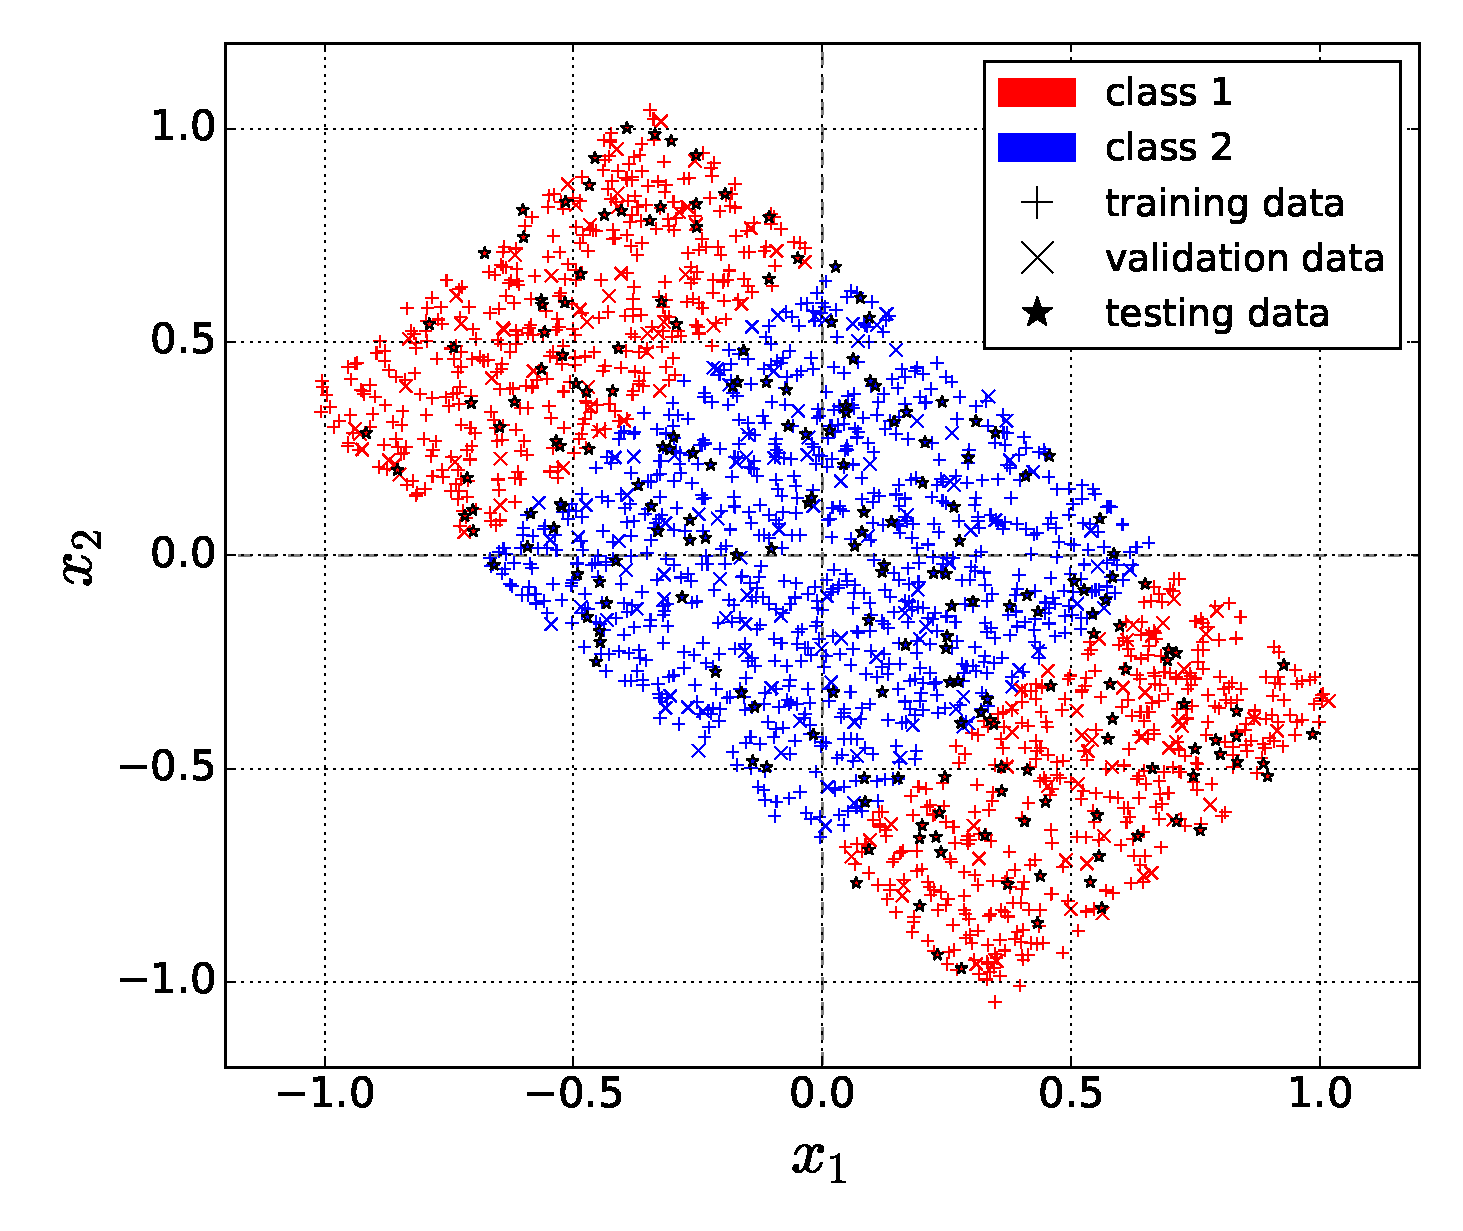
\includegraphics[width=\textwidth]{dataset_xor.eps}
\caption{The XOR dataset.}
\label{fig:examples:dataset_xor}
\end{figure}

\section{2D-problem B: Unbalanced Features} \label{sec:dataset_unbfea}
Karnin data...

\begin{figure}[H]
\centering
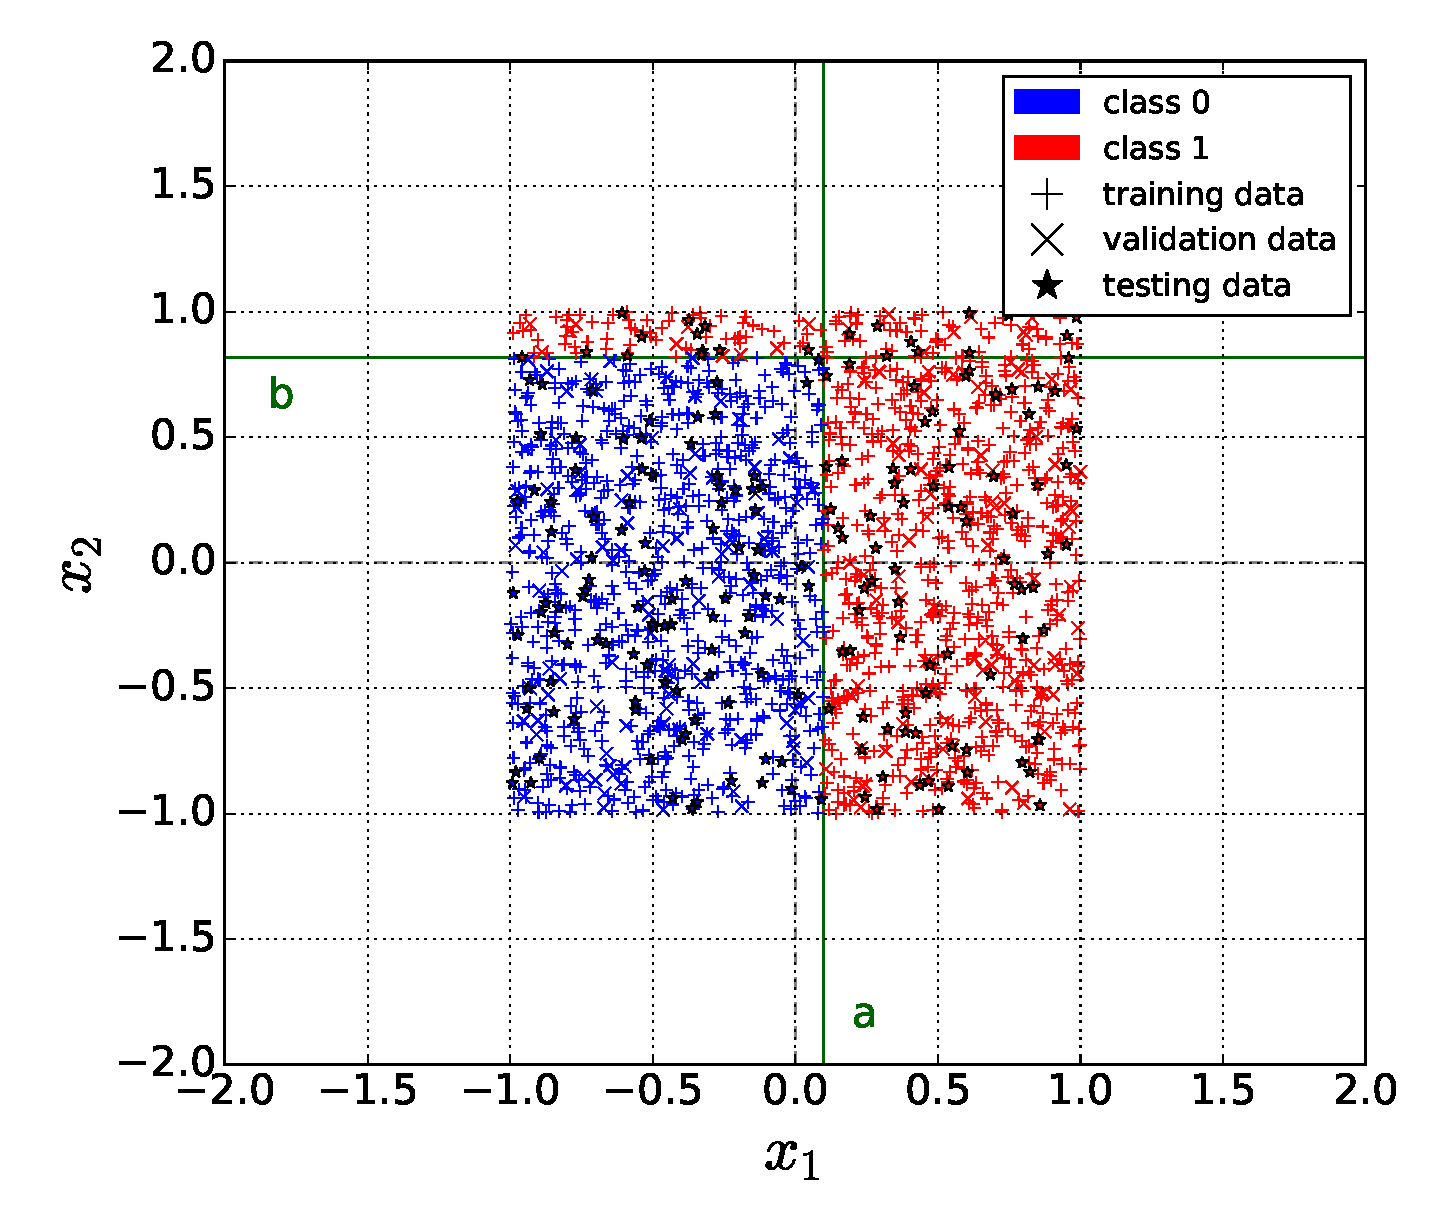
\includegraphics[width=\textwidth]{dataset_unbfea.eps}
\caption{The dataset with unbalanced features.}
\label{fig:examples:dataset_unbfea}
\end{figure}

\section{Rule-plus-Exception Problem} \label{sec:dataset_rpe}
RPE data...

\section{The Train Problem} \label{sec:dataset_train}
The Michalski's train problem...

\begin{figure}[H]
\centering
\includegraphics[width=\textwidth]{michalski_train_problem}
\caption{Michalski's train problem.}
\label{fig:examples:dataset_train}
\end{figure}

\section{Handwritten digits (MNIST)} \label{sec:dataset_mnist}
MNIST data... \citep{online:mnist}

\section{Phonemes (speech data)} \label{sec:dataset_phonemes}
PHONES data...
